\documentclass[11pt,a4paper]{article}
%\usepackage[toc,page]{appendix}
\usepackage{graphicx}
\usepackage[a4paper]{geometry}
\usepackage{xcolor}
\usepackage{fancyhdr}
\usepackage{float}
\usepackage{setspace}
\usepackage[absolute]{textpos}
\usepackage{epstopdf}
%\usepackage[]{mcode} 	% To include matlab code
\usepackage{capt-of}
\usepackage{enumerate}
\usepackage{lastpage}
\usepackage{booktabs}
\usepackage{longtable}
\usepackage{array}
\renewcommand{\arraystretch}{1.5}

\usepackage[english]{babel}
\usepackage[utf8]{inputenc}
\usepackage{amsmath}
\usepackage{amsfonts}
\usepackage{graphicx}
\usepackage[colorinlistoftodos]{todonotes}
\usepackage{algorithm}
\usepackage{algpseudocode}

\usepackage{amsmath}
\usepackage{algorithm}
%\usepackage[noend]{algpseudocode}
\makeatletter
\def\BState{\State\hskip-\ALG@thistlm}
\makeatother

\usepackage{amsmath}
\usepackage{amsfonts}
\usepackage{amssymb}
\usepackage{eurosym}

% Header
\setlength{\headheight}{30pt}
\newgeometry{top=2.5cm, bottom = 1.5cm, left=2cm, right=2cm}
\pagestyle{fancy} 
\lhead{\includegraphics[height=0.8cm]{figures/{tue_logo}.png}}
%\lfoot{Group 4 - ``CASE"-HENK}
\cfoot{~}
\rfoot{Page \thepage ~of \pageref{LastPage}}

\usepackage{cleveref}
% Change cleveref reference eq. to equation same for figure
\crefname{equation}{equation}{equations}
\crefname{figure}{figure}{figures}
\crefname{table}{table}{tables}

% Change Section numbering to Problem 1
%\renewcommand{\thesection}{Problem \arabic{section}.}

\begin{document}
%\begin{titlepage}
%\vspace*{100pt}
%\begin{figure}
%\centering
%\includegraphics[width=0.5\textwidth]{figures/TUelogozondertekst}
%\end{figure}
%\begin{center}
%{ \huge \bfseries 4AT100 Automotive Systems Engineering Project\\[0.4cm] }
%\textsc{\Large Concept Project Plan}\\[0.5cm]
%
%\end{center}
%
%\vfill
%
%\renewcommand{\arraystretch}{1}
%
%\begin{flushleft} \large
%\begin{tabular}{l}
%Project Coordinators:\\
%Dr.Ir. A. van de Mortel-Fronczak (Asia) \\
%Dr.Ir. I. Barosan (Ion) \\
%\end{tabular}
%\end{flushleft}
%
%\begin{flushleft} \large
%\begin{tabular}{l l l l}
%Tutor: & & & \\
%L. Kefalidis (Lazaros) & & & \\
%& & & \\
%Authors:\hspace{30mm} 	& \hspace{35mm}	& \hspace{55mm} 	    		& 			\\
%S. Forno (Simone) 		& ​0978942		& T. de Mor\'ee (Tim)			& 0944052 	\\
%R.M.A. Goris (Rob) 		& 0808822		& T.M.A. van de Wiel (Thijs)	​& 0824530 	\\
%B.S. Haarsma (Bouke) 	& 0751757​		& H. Wils (Hielke) 				& 0807014 	\\
%\end{tabular}
%\end{flushleft}
%
%\begin{flushleft} \large
%\begin{tabular}{l}
%MSc. Programme Automotive Technology \\
%Eindhoven University of Technology \\
%\end{tabular}
%\end{flushleft}
%
%\begin{flushleft} \large
%\begin{tabular}{l}
%\today \hspace{8.4cm} Group 4 ``CASE"-HENK \\
%\end{tabular}
%\end{flushleft}
%
%\renewcommand{\arraystretch}{1.5}
%
%\end{titlepage}

\newgeometry{top=2.5cm, bottom = 3cm, left=2cm, right=2cm}

%\newpage
%
%\setcounter{tocdepth}{2}
%
%\tableofcontents
%\newpage


%------------------------------------------------


\section{Configuration of Amcl parameters}

The results so far (see update document of 12{\_}11) did show deviations in the pose, drifting by some value as soon as the end of a straight line has been reached. This is probably due to errors in the motion model, which needs to be compensated by tuning proper parameters. \textbf{Amcl} does infact strongly rely on \textbf{odometry} and \textbf{sample motion model}, hence if errors in the odometry occurs (the error in the odometry is always presence due to the noise), this will just accumulate. \\
The \textbf{Kinematic motion} model in use will be \textbf{odometry motion model}; there is also a velocity motion model, not in use by AMCL. The latter tend to be less accurate (for all details see book Probabilistic Robotics p. 96).

\begin{center}
\captionof{table}{AMCL parameters}
\begin{tabular}{| m{12em} | m{13em}|} 
\hline
alpha1 & Specifies the expected noise in odometry's rotation estimate from the rotational component of the robot's motion, has an effect on Figure 1.b\\
\hline
alpha2 & same as alpha1, but for the translational component\\
\hline
alpha3 & Specifies the expected noise in odometry's translation estimate from the rotational component of the robot's motion, Figure 1.c \\
\hline
alpha4 & same as alpha3, but for the translational component\\
\hline
\end{tabular}
\end{center}

\begin{figure}[H]
	\center
	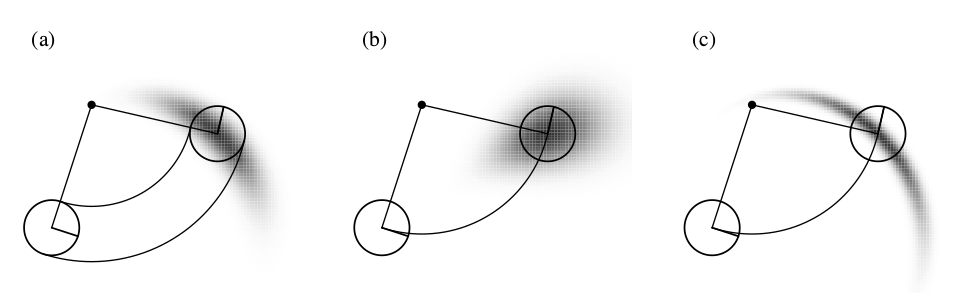
\includegraphics[width=.7\textwidth]{figures/motion_models.png}
	\caption{Velocity motion models for different noise parameters settings. Figure .b shows large translational error and small angular error, Figure .c large angular errors and small translational error}.
	\label{fig:models}
\end{figure}

\subsection{AMCL with GMapping map}

This case presents a deviation (a translation) due to angular drift; therefore the first parameter that should be tuned is \textbf{alfa4}. The strategy is to put all alfas to a small value, then increase it progressionally till the optimal. \\
The particles of the filter are fixed to \textbf{6000,9000}.

See this link for an answer: https://answers.ros.org/question/227811/tuning-amcls-diff-corrected-and-omni-corrected-odom-models/

\newpage
\begin{center}
\captionof{table}{alfa parameters and results}
\begin{tabular}{| m{12em} | m{13em}|} 
\hline
\textbf{Parameters} & \textbf{Results} \\
\hline
 alfa4=0.05 &  Just changing this alone did not produce considerable results at all\\
\hline
 alfa4=0.05, alfa3=0.05 &  Also this combinations does not have an effect on the bearing error. The alfas here have been changed to a factor of 20.\\
\hline
 alfa3,4=default=2, alfa1,2=0.05 & Also no result in here \\
\hline
all alfas to 0.1 & Also did not see nothing relevant\\
\hline
alfa1=0.005, alfa2=0.005, alfa3=0.010, alfa4=0.005& No satisfactory results\\
\hline
alfas=0.0001 & works now, I loose global localization property with such a small values, if calling the global localization service. \\
\hline
\end{tabular}
\end{center}

\begin{center}
\captionof{table}{Starting from the corrected alfas = 0,0001, higher progressively alfa3, alfa4 till the optimal}
\begin{tabular}{| m{12em} | m{13em}|} 
\hline
\textbf{Parameters} & \textbf{Results} \\
\hline
alfa3,4=0,001 (try a factor of 10 higher) & Still get considerably good results \\
\hline
\hline
alfa3,4=0,01 (try a factor of 10 higher) & With those value the error is not anymore bounded to the 5 centimeters, hence we keep as a good result the value of before. \\
\hline
\end{tabular}
\end{center}

\begin{center}
\captionof{table}{Update min a/d}
\begin{tabular}{| m{12em} | m{13em}|} 
\hline
\textbf{Parameters} & \textbf{Results} \\
\hline
& \\
\hline
\hline
\hline
\end{tabular}
\end{center}


\end{document}


% == TABLE ==
%begin{table}[h!]
 % \centering
  %\caption{Caption for the table.}
 % \label{tab:table1}
 % \begin{tabular}{ccc}
 %   \toprule
  %  Some & actual & content\\
   % \midrule
   % prettifies & the & content\\
   % as & well & as\\
  %  using & the & booktabs package\\
  %   \bottomrule
  %\end{tabular}
%\end{table}


% === ALGORITHM == 

{\_}

\iffalse % multi-comment tool
\begin{algorithm}[!h]
   \caption{Kirsch, Rohig algorithm}
    \begin{algorithmic}[1]
    	\State $St-1 = St$
        \For{$i = 1$ to $N$} \Comment{With N the number of particles in the filter set by maxparticle parameter}
            \State $Spread $ $particles$ $in$ $the$ $anchorbox$ $with$ $equations$ $1)$ $and$ $2)$ $of$ $[3]$ \Comment{This step is called $Global$ $Localization$}
            
            \State $xt[n] = p(xt|xt-1,ut)$ \Comment{Motion update - sample the particles from the motion update of the robot and move forward to estimate the error model functions}
            
        	\State $wt[n] = p(dnanoLOC|si)*p(dlaser|si)$ \Comment{Measurement update - si are the particles set with i the i-th index}
        	\State $St = St + <xt,wt>$ \Comment{add the state and weight to the total state space}
        	
        	\State $Perform$ $resampling$
        \EndFor
    \State $Return$ $St$

\end{algorithmic}
\end{algorithm}
\fi


\iffalse

\begin{figure}[!htb]
    \centering
    \begin{minipage}{.5\textwidth}
        \centering
        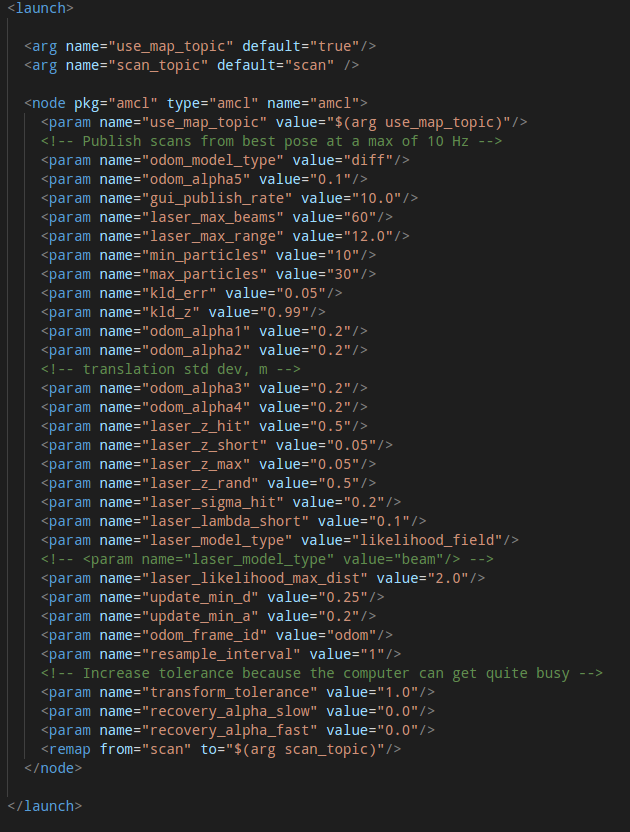
\includegraphics[width=0.7\linewidth, height=0.2\textheight]{figures/amcl_param}
        \caption{The $amcl$ tunable parameters}
        \label{fig:amcl_param}
    \end{minipage}%
    \begin{minipage}{0.5\textwidth}
        \centering
        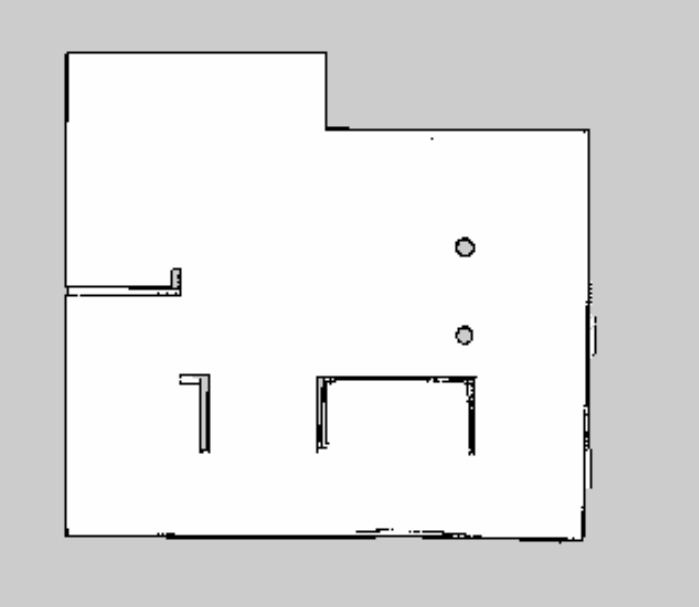
\includegraphics[width=0.7\linewidth, height=0.2\textheight]{figures/my_amcl_gmapping}
        \caption{Result of the Gmapping for the simple indoor environment}
        \label{fig:myamcl_map}
    \end{minipage}
 \end{figure}
 
 
 
\begin{figure}[!htb]
	\center
	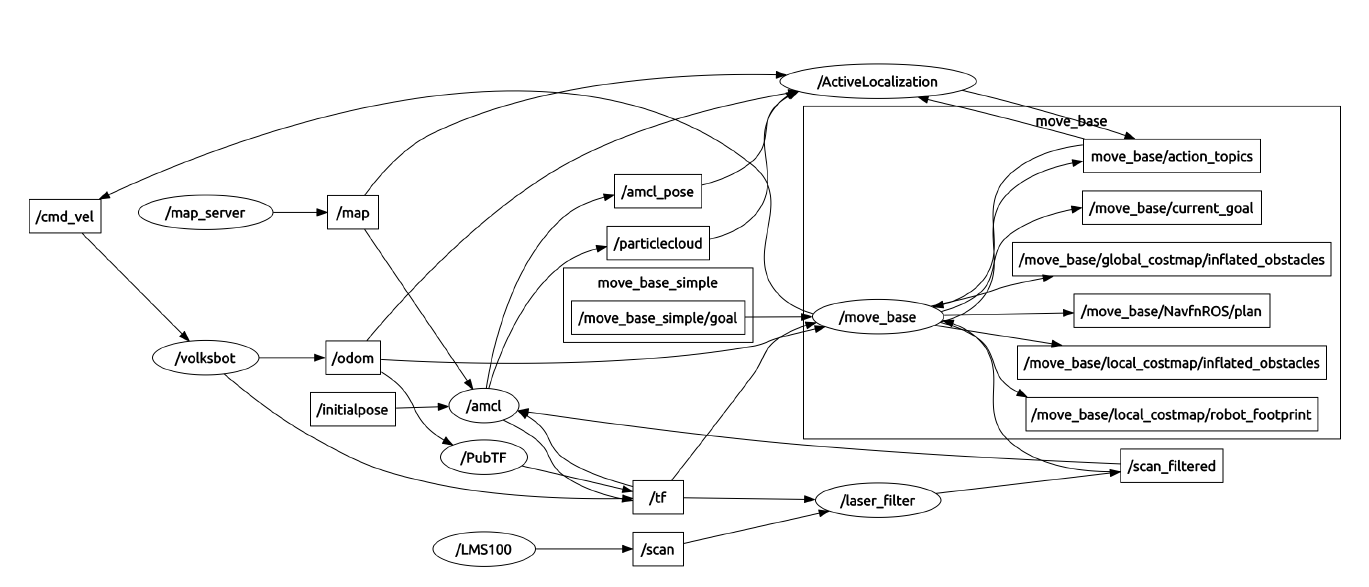
\includegraphics[width=1\textwidth]{figures/active_localization_node.png}
	\caption{An example of an active localization node}
	\label{fig:active_locnode}
\end{figure}


% underscore symbol {\_}

\begin{center}
\captionof{table}{}
\begin{tabular}{| m{12em} | m{13em}| m{12em}|} 
\hline
& &  \\
\hline
\end{tabular}
\end{center}

\fi